% chap2_structure.tex — 構造
\section{アクチュエータ構造と設計指針}

本章では,提案する静電薄膜MEMSアクチュエータの構造および設計上の要点を示す。
図\ref{fig:stack}に示すように,本デバイスは
Si(100)基板上に Poly-Si(0.2\,\textmu m)/ALD-Al$_2$O$_3$(60\,nm)/
Gap(0.8--1.0\,\textmu m)/SiN$_x$(0.8\,\textmu m, +150\,MPa)/
Pt-Ti(100/20\,nm)/Parylene-HT(1.0\,\textmu m)/PEG-SAM
を積層した平板型構造である。

\subsection{基板とキャビティ構成}
従来は機械的安定性を重視して Si(111) 基板が多用されてきたが,
本研究では CMOS後工程との整合性とエッチング制御性を優先し,
\textbf{Si(100)} を採用した。
Si(100) は異方性エッチング(KOHまたはXeF$_2$)により
平坦な底面キャビティを形成でき,背面開口の位置制御精度が高い。
これにより,ダイアフラムの有効面積を正確に定義し,
膜応力の再現性を向上できる。

\subsection{絶縁層と電極構成}
下部電極の上には,ALD-Al$_2$O$_3$(60\,nm)を介在させた。
ALD (Atomic Layer Deposition) による原子層精度の成膜は
側壁までコンフォーマルに被覆するため,
電界集中を緩和し絶縁破壊電界を 8--10\,MV/cm まで高められる。
上部膜は SiN$_x$(0.8\,\textmu m)で構成し,
LPCVD 条件で引張応力を +150\,MPa に制御することで,
変位応答の直線性と Pull-in 安全率を両立させた。
その上に形成された Pt/Ti(100/20\,nm) 電極は,
高導電かつ生体適合性に優れ,Parylene-HT 膜との密着性を確保する。

\subsection{表面保護膜と生体整合性}
上面保護膜には Parylene-HT(1.0\,\textmu m)を用い,
水分吸収が少なく,かつ低表面エネルギーで
電気絶縁と耐薬品性を両立する。
さらに,その表面を PEG-SAM (polyethylene glycol self-assembled monolayer)
で修飾することにより,タンパク質や核酸の非特異吸着を抑制し,
生体分子活性の保持を図った。

\subsection{静電設計と安全率評価}
静電駆動の力学的モデルは,
\begin{equation}
F=\frac{1}{2}\varepsilon_0\varepsilon_r\frac{A V^2}{(g-x)^2}, \qquad
V_{\mathrm{PI}}=\sqrt{\frac{8kg^3}{27\varepsilon_0\varepsilon_r A}},
\label{eq:pullin}
\end{equation}
で与えられる。
ここで,$A$ は駆動電極面積,$g$ は初期ギャップ,
$k$ は膜の等価ばね定数である。
設計値 $A=(25\,\textmu\mathrm{m})^2$, $g=0.8\,\textmu$m, $k=150\,\mathrm{N/m}$
を代入すると,Pull-in 電圧 $V_{\mathrm{PI}}\approx100$\,V が得られる。
45\,V 駆動時には $x=0.10$--$0.12\,\textmu$m の変位が得られ,
安全率 $>2$ を維持できる。
この動作領域では,静電力と膜応力がほぼ線形に釣り合うため,
アクチュエータ出力は安定で熱依存性も小さい。

\subsection{設計指針のまとめ}
以上の設計により,
(1) \textbf{Pbフリー・低温整合}(Al$_2$O$_3$/SiN$_x$ベース),  
(2) \textbf{低電圧駆動・高信頼絶縁}(45\,V typ, 100\,V max),  
(3) \textbf{生体適合・低吸着表面}(Parylene-HT/PEG-SAM),  
を同時に達成した。
これにより,電気・機械・化学の複合設計に基づく
「穏やかに動く精密アクチュエータ」の
実用的アーキテクチャが確立された。

\begin{figure}[t]
\centering
\resizebox{0.95\columnwidth}{!}{%
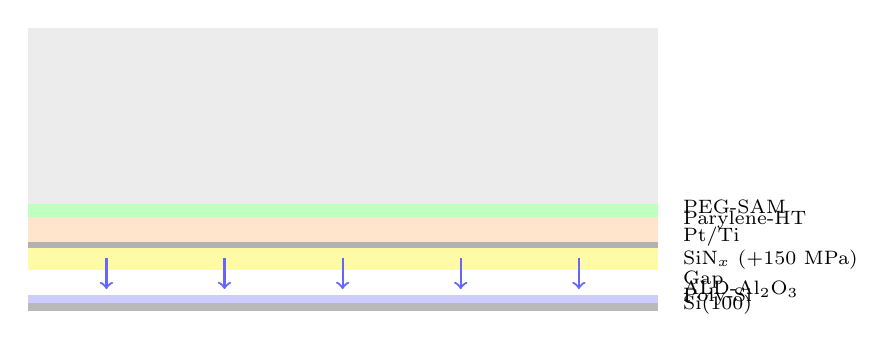
\begin{tikzpicture}[x=1mm,y=2mm]
  \fill[gray!15] (0,0) rectangle (80,-18); % Si(100)
  \fill[gray!55] (0,-18) rectangle (80,-17.5); % Poly-Si
  \fill[blue!20] (0,-17.5) rectangle (80,-17.0); % ALD-Al2O3
  \fill[white] (0,-17.0) rectangle (80,-15.4); % Gap
  \fill[yellow!35] (0,-15.4) rectangle (80,-14.0); % SiNx
  \fill[gray!60] (0,-14.0) rectangle (80,-13.6); % Pt/Ti
  \fill[orange!20] (0,-13.6) rectangle (80,-12.0); % Parylene-HT
  \fill[green!25] (0,-12.0) rectangle (80,-11.2); % PEG-SAM
  \foreach \x in {10,25,40,55,70}{
    \draw[->,blue!60,thick] (\x,-14.6)--(\x,-16.6);
  }
  \node[anchor=west,font=\scriptsize] at (82,-17.6){Si(100)};
  \node[anchor=west,font=\scriptsize] at (82,-17.1){Poly-Si};
  \node[anchor=west,font=\scriptsize] at (82,-16.6){ALD-Al$_2$O$_3$};
  \node[anchor=west,font=\scriptsize] at (82,-16.0){Gap};
  \node[anchor=west,font=\scriptsize] at (82,-14.7){SiN$_x$ (+150 MPa)};
  \node[anchor=west,font=\scriptsize] at (82,-13.3){Pt/Ti};
  \node[anchor=west,font=\scriptsize] at (82,-12.2){Parylene-HT};
  \node[anchor=west,font=\scriptsize] at (82,-11.4){PEG-SAM};
\end{tikzpicture}}
\caption{提案静電薄膜MEMSアクチュエータの積層構造概念図。電界線を青矢印で示す。}
\label{fig:stack}
\end{figure}
